\subsection{Theory}

\subsubsection{Noise}

One of the most funadmental tools used in PCG is noise.
Noise is the concept of random values, often represented using a 2D or 3D matrix of real numbers.
The two major types of noise that are commonly used are \textit{value noise} and \textit{gradient noise}.

\textit{Value noise} is constructed by first randomizing the values of a few lattice points in the matrix, and then interpolating these values for intermediate points.
Bilinear and bicubic interpolation are common in practice since they are fast to compute.
Value noise is simple to implement, but it has several disadvantages.
First off, the noise ends up with a grid-like structure because of the lattice points.
This is often undesired since it creates arbitrary patterns in the noise.
Furthermore, neighboring lattice points may greatly differ in values which can result in sudden changes in steepness.

\textit{Gradient noise} solves the problems with value noise by first constructing slopes, and then sample values from those.
By interpolating slopes (or gradients) that already are smooth, we ensure that not only changes in values are smooth but also the \textit{rate of change} between them.
This causes nearby points to be of similar random values, while points far apart to be unrelated.

Both types of noise can be represented with intensity maps as seen in figure~\ref{fig:noisetypes}.
An intensity map is a bitmap image where each pixel represents the value of the underlying noise.
White pixels indicate maximum values, and black pixels represents minimum values.
These maps can be used to represent many things including heights, in which case they are referred to as \textit{heightmaps}.
They can also be used to create smooth blending between textures.

\begin{figure}[h!]
  \centering

  \begin{subfigure}[b]{0.30\textwidth}
    \frame{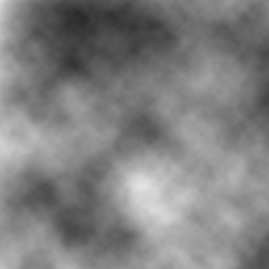
\includegraphics[width=\textwidth]{figure/value_noise.png}}
    \caption{Value noise. \cite{value_noise}}
  \end{subfigure}
  \quad
  \quad
  \quad
  % NOTE(anton): image generated from https://cpetry.github.io/TextureGenerator-Online/
  \begin{subfigure}[b]{0.30\textwidth}
    \frame{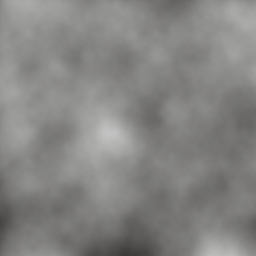
\includegraphics[width=\textwidth]{figure/heightmap.png}}
    \caption{Gradient noise.}
  \end{subfigure}

  \caption{Examples of value noise and gradient noise represented using intensity maps. Notice how the value noise has cross-like patterns.}
  \label{fig:noisetypes}
\end{figure}

A commonly used implementation of gradient noise is \textit{Perlin noise}, which later evolved into an improved version called \textit{simplex noise}.
Ken Perlin introduced \textit{Perlin noise} in 1985 with the intention to produce more natural looking textures \cite{perlin_noise}.
Although \textit{simplex noise} is the improved version, the two terms are often used interchangeably. The idea of \textit{simplex noise} is described in great detail by Stefan Gustavson in his paper \textit{Simplex noise demystified} \cite{simplex_noise}.
He also mentions several technical advantages with the technique.
This subsection describes different ways of generating procedural content, for example Gradient noise and L-systems.

\subsubsection{Search-based}
One method for generating content is using a \textit{search-based} approach.
This often involves using an evolutionary algorithm with some stochastic search/optimization algorithms to determine a solution with desired qualities.
The general idea is that a for a given design problem we can find an acceptable solution by ``searching'' for it within the solution space.
When iterating over the solutions they are tweaked according to an evaluation function that keeps the changes which make the solution(s) ``better'' and discards any harmful changes.
By iterating and tweaking one or many of possible solutions we will eventually arrive at a desired solution.
% http://pcgbook.com/wp-content/uploads/chapter02.pdf

\subsubsection{Machine learning}
Machine learning(ML) is another method that can be used to procedural generate worlds. 
This could be useful when it is hard to explicity create logic when there is many parameters at play.
There is a lot of parameters one could take into account when generating a city, and ML could be a solution.

\subsubsection{L-System}
An L-system is a type of formal grammar typically used in procedural generation.
It is built up of strings which under a set of constraints recursively grow larger and more complex with each iteration.
These strings are then used to build geometric structures.
L-system grammars are defined of three parameters which can be denoted as following:

\begin{itemize}
  \item V        --- The alphabet, consists of symbols which are referred to as constants or variables.
  \item $\omega$ --- axiom, an initial symbol from V which defines the initial state of the system.
  \item P        --- Production rules, these are the constraints which determines how variables should be replaced.
\end{itemize}

The variables are replaced with a mix of variables and constants, which recursively leads to a very large and complex resulting set.
One special attribute  for L-systems is that rather than the constants and variables being evaluated one by one in a left to right manner they are all evaluated in parallel.
A special case of L-systems is referred to as \textit{Stochastic bracketed L-systems}.
A grammar being stochastic means that the there are a number of production rules which can be applied to each variable that all have different probability of occurring.
Bracketed means that we have a push/pop structure where a [ means that we push a value, storing it, and a ] means that we return to where we pushed most recently.
The reasoning for being able to return to a previously stored point in the string is that it results in less continuous generation.
This is well expressed in the book Procedural Content Generation In Games[p.77], ~\cite{PCG_in_games} where they describe the limitations of non-bracketed L-systems in the following way:
"While interpreting L-system-generated strings as turtle instructions allows us to draw complex fractal shapes, we are fundamentally limited by the constraint that the figures must be drawable in one continuous line—the whole shape must be drawn “without lifting the pencil”".
